\graphicspath{ {./figuresAnalysis} }
\section{Analyse fonctionnel}
\subsection{Besoin}
Afin d'être sûre de commencer dans la bonne direction nous devons définir clairement les besoins auquel notre capteur devra répondre. Comme décrit précédemment, le besoin principal est la prévention du développement de maladie. Il existe des modèles empiriques qui se basent sur le temps d'humidité sur la feuille. Cette variable est difficile à déterminer par les données météo classique (humidité, température, vents etc). Le recours à un capteur d'humectation est utile dans ce cas là.
Un autre besoin est pour l'aide aux traitement. La plupart des traitements chimiques d'une plantation doivent être effectués lorsque les feuilles sont sèches. Un capteur d'humectation doit permettre de fournir cette information rapidement.  

\begin{figure}[!ht]
 \centering
 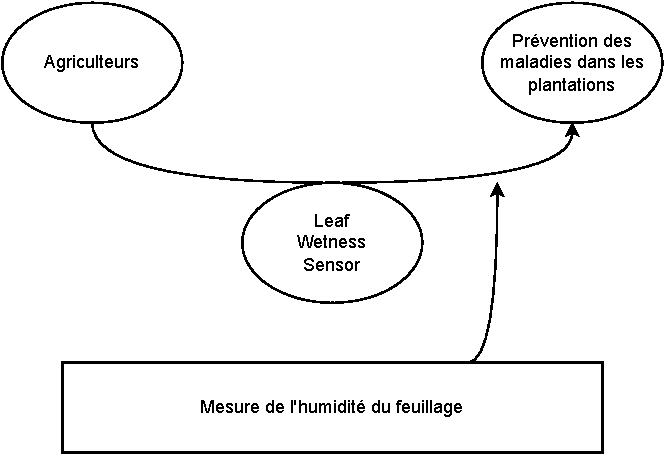
\includegraphics{DiagrammeCorne.drawio.pdf}
 \caption{Le besoin principale exprimé sous la forme d'un diagramme bête à cornes.}
\end{figure}

\subsection{Fonction principale et contrainte }

Pour répondre aux besoins, la fonction principale sera de mesurer l'humectation des feuilles. Cette fonction s'accompagne de plusieurs contraintes apportées par l’environnement dans lequel s'inscrit le capteur. Pour être sûre de n'en oublier aucune, nous nous aidons d'un diagramme pieuvre. 

\begin{description}
 \item[FC1] Il est développé dans le cadre du projet JDC Smart Farming. Il devra être compatible avec le système déjà créé. 
 \item[FC2] Il sera déployé dans des plantations avec une batterie comme source d'énergie. La consommation doit être contrôlée.   
 \item[FC3] En extérieur la météo peut faire varier l’environnement du capteur. Il devra être robuste à ces changements pour qu'il n’influence pas les mesures.
 \item[FC4] Les intempéries que subira le capteur ne doivent pas l’endommager ou compromettre les mesures.
 \item[FC5] Dans les plantations, il y a régulièrement des tracteurs et des machines qui passent entre les plantes. Le capteur ne doit pas gêner ou être gêner par ces passages. Sa taille doit être contrôlée.
 \item[FC6] L'installation et la maintenance pourra être faite par des agriculteur sans formation technique. Le capteur doit être simple d'installation et de maintenance.
 \item[FC7] Le capteur est développé pour être commercialisé. Il doit répondre aux norme et être certifié.
\end{description}

\newpage

\begin{figure}[!ht]
 \centering
 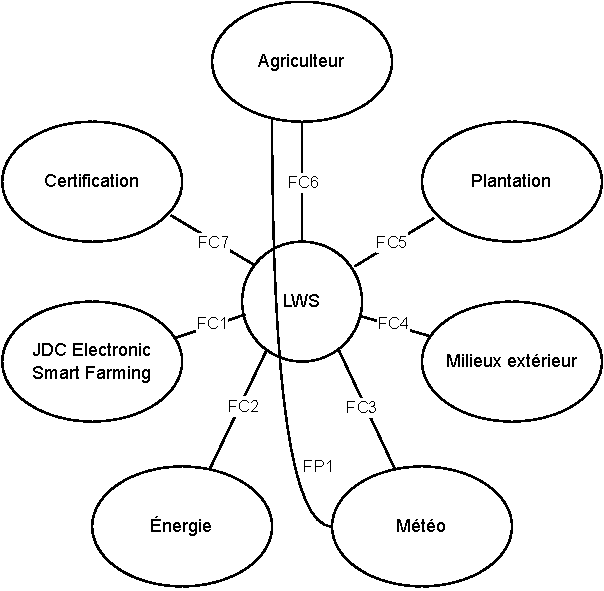
\includegraphics{DiagrammePieuvre.drawio.pdf}
 \caption{Fonctions principales et contraintes sous la forme d'un diagramme pieuvre}
\end{figure}

Après avoir énoncé la fonction principale et toutes les contraintes nous pouvons définir des critères pour chacune d'elles ainsi que des nivaux qui répondent à ces critères. Cela nous permet de construire le cahier des charges auquel nous nous référons pour la conception. 

\paragraph{FP1}
La mesure d'humectation des feuilles se fera au travers d'une mesure de l'humidité relative d'une surface. Elle se donne en pourcentage tel que 0\% correspond à un feuille totalement sèche et 100\% la feuille est entièrement recouverte d'eau. Puisque nous ne connaissons pas encore les performances de notre capteur nous utiliserons la résolution maximale qu'autorise la structure de registre de JDC pour ce type de capteur. La valeur sera stockée sur 1 octet non signé avec une résolution de 0.5\%. La précision est calqué sur la résolution et donne une valeur de 0.25\%. Ces valeur sont très optimistes et nous nous resservons le droit de les changer après une évaluation des performance du capteur plus tard dans le développement. 

\paragraph{FC1} \label{fc1}
L’environnement Smart Farming JDC se compose d'un émetteur LoRa auquels sont reliés plusieurs capteurs au travers d'un bus I2C. Pour que notre capteur soit compatible, il doit impérativement répondre à plusieurs critères. L'interface de sortie doit être évidement un I2C. La structure des registres accessibles est normalisé pour que l’émetteur puisse lire correctement les valeurs afin de les transmettre. Un temps maximal de mesure est défini. Il représente le temps entre le démarrage du capteur jusqu'à que les valeurs de la mesure soit prête. Le capteur devra être câblé sur le connecteur commun à tous les capteurs JDC. Pour finir, l'alimentation fourni par l'émetteur est de 3.3V le capteur devra fonctionner à cette tension.

\paragraph{FC2}
La source d'alimentation du capteur sera une batterie situé aux niveau de l'émetteur. Tous les capteurs d'un même émetteur partage donc la même source. Les capteurs ne sont pas alimentés entre deux mesures. Nous n'avons pas besoin de nous préoccuper de la consommations au repos. En marche, le courant, que nous prendrons comme critère, ne doit pas dépasser 1mA. Ce chiffre avait été calculé par rapport au nombre maximal de capteur ,la capacité de la batterie et l'autonomie souhaité.  

\paragraph{FC3}
Le facteur métrologique qui pourra le plus fausser nos mesures est l'humidité de l'air. Si l'air est chargée en eau, sa constante diélectrique changera et pourra impliquer un augmentation de la capacité alors que la surface est complètement sèche. Pour que ce phénomène n’influence en aucun cas nos mesures, le delta de capacité doit être inférieur à la précision. Cette variation devra être contrôlé et mesurée car elle pourrait dégrader la précision du capteur.   

\paragraph{FC4}
L'utilisation extérieur du capteur nécessite qu'il soit étanche aux intempéries. Avec la norme IP65 comme objectif, le capteur sera suffisamment protéger des plus grosses pluies ainsi que des traitements pulvérisés sur les cultures.    

\paragraph{FC5}
Pour s’intégrer aux mieux dans les plantations le capteur ne devra pas être trop volumineux. Nous prendrons arbitrairement une envergure maximum de 20 cm. Cela correspond à une moyenne des capteur existant sur le marché.

\paragraph{FC6}
La facilité d'installation a déjà été pensée et est garantie par la contrainte \textbf{FC1}.

\paragraph{FC7}
Pour être proposé sur le marché le capteur doit être certifié. Il doit possédé le CE pour être distribué en Europe et une certification de compatibilité électromagnétique pour garantir que le capteur respecte les normes en vigueur.  

\bigskip
Le cahier des charge résume tous les critères et leur niveau pour chaque contrainte.

\begin{table}[!h]
\begin{center}
\resizebox{\columnwidth}{!}{%
\begin{tabular}{|l|l|p{5cm}|l|}
\hline
 & \textbf{Fonctions} & \textbf{Critères} & \textbf{Niveaux}\\
\hline
\textbf{FP1} &Mesurer l'humectation des feuilles & Mesure d'humidité relative d'une surface & RH de 0\% à 100\%  résolution de 0.5\%  précision +- 0.25\%\\
\hline
\multirow{5}{*}{\textbf{FC1}} & S'intégrer dans l'environnement Smart Farming JDC & Interface  de sortie I2C & Baud rate 100KHz. Adresse configurable\\\cline{3-4}
 &  & Structure de registre normalisé, & (voir doc JDC)\\\cline{3-4}
 &  & Démarrage de la mesure et acquisition après un temps. & 50ms pour la capture de la mesure\\\cline{3-4}
 &  & Connecteur JDC & Sortie 4 fil avec  VCC,GND,SDA,SCL\\\cline{3-4}
 &  & Alimentation normalisé & Tesion 3.3V\\\cline{3-4}
\hline
\textbf{FC2} & Consommer peu d'énergie & Courant maximum établit en fonctionnement & 1 mA\\
\hline
\textbf{FC3} & Eviter les faux positifs du à la météorologie & L'humidité de l'air ne doit pas influencer la mesure & L'incidence de RH de l'air < précision (0.25\%)\\
\hline
\textbf{FC4} & Résister aux milieux extérieurs & Le capteur est protégé des intempéries et supporte une utilisation extérieur & Etanche IP65\\
\hline
\textbf{FC5} & S'intègrer dans les plantations & La taille du capteur ne doit pas gêner l'exploitation des plantations & Envergure maximum de 20cm\\
\hline
\textbf{FC6} & Etre facile d'installation & Le capteur doit pouvoir être installer par des agriculteurs sans formation technique & Système d'attache et un seul connecteur à brancher\\
\hline
\textbf{FC7} & Etre Certifié & Le capteur doit être certifié pour être proposé sur le marché & Certification EMC,CE\\
\hline
\end{tabular}
}
\end{center}
\caption{Cahier des charges}
\end{table}

\newpage

\subsection{Architecture du système}

En nous basant sur le cahier des charges, nous pouvons commencer à concevoir l'architecture de notre capteur. Pour nous aider dans cette tâche nous utiliserons un diagramme FAST. Il nous permettra méthodiquement de faire la liste de tous les éléments nécessaires au bon fonctionnement du capteur.

\begin{figure}[!ht]
 \centering
 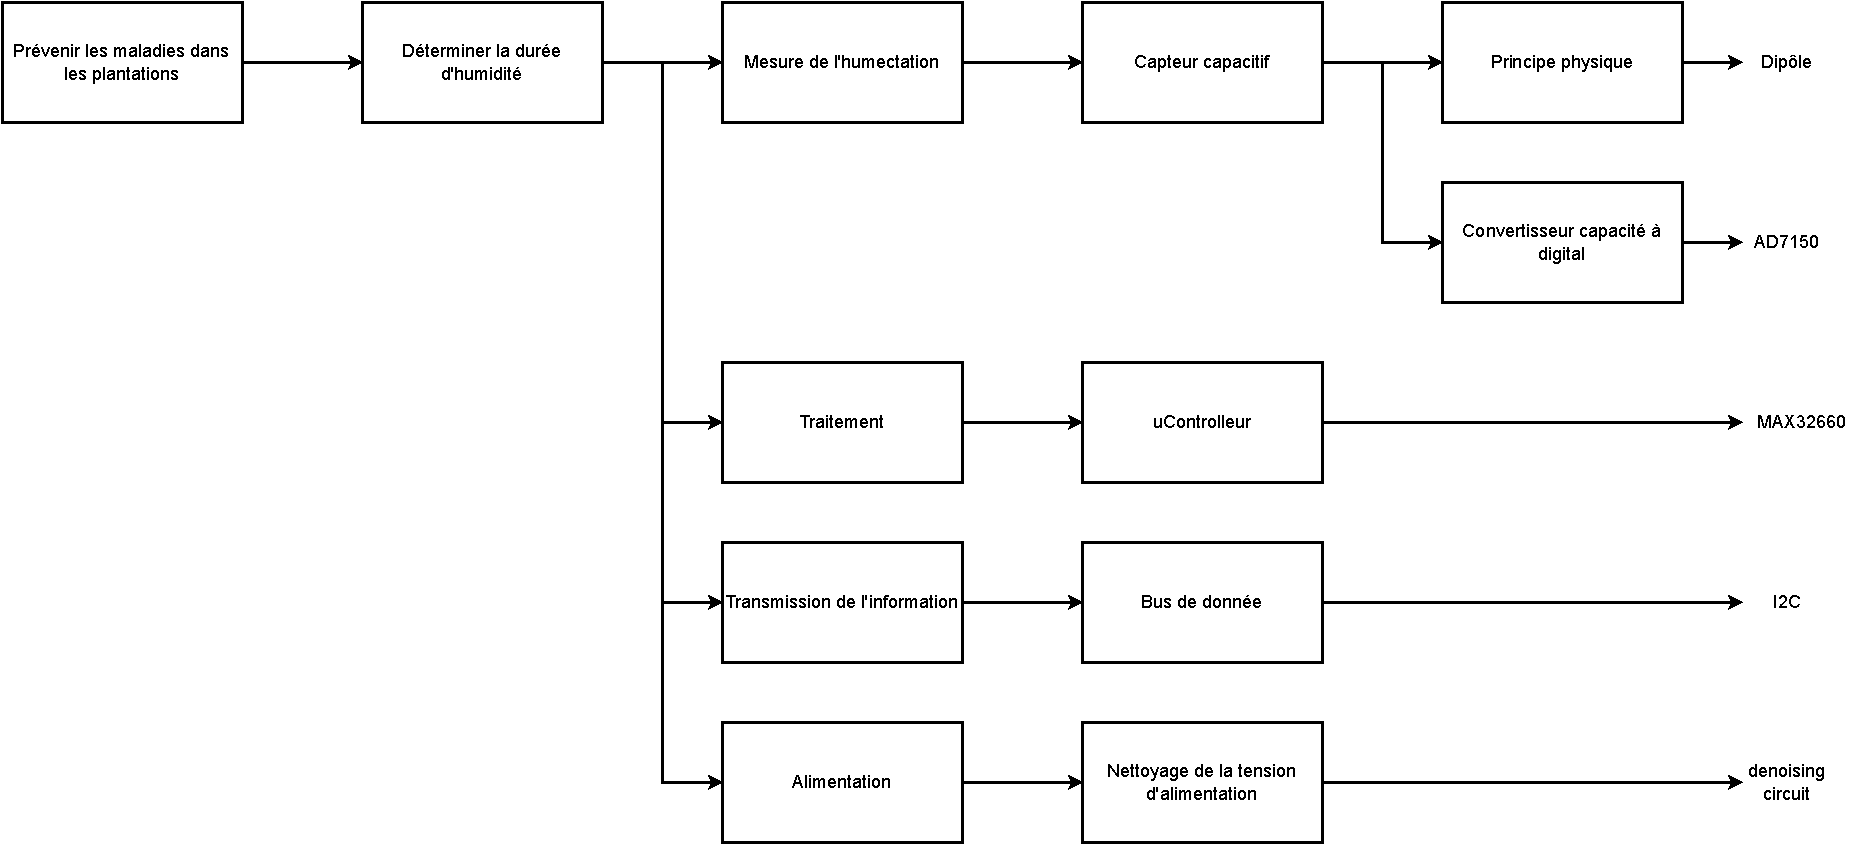
\includegraphics[width=16cm]{DiagrammeFAST.pdf}
 \caption{Diagramme FAST}
\end{figure}

Plusieurs choix techniques ont été fait pendant cette phase d'architecture. Le MAX32660 a été choisi comme micro-contrôleur. JDC l'utilise déjà dans ses capteurs. Plusieurs librairies ont déjà été créés pour intégrer le capteur dans l’environnement JDC ce qui facilitera le développement. Le micro-contrôleur a tous les périphériques que nous avons besoin et est prévu pour la faible consommation. Il ira très bien dans notre application.


l'AD7150 a été choisi parmi les différents convertisseurs capacitifs présentés pendant l'état de l'art. La sélection c'est fait sur la consommation des circuits intégrés. l'AD7745 et le FDC1004 ont une consommation en travail de  \SI{900}{\micro\ampere}. C'est beaucoup trop si on prends en compte le fait qu'un micro-contrôleur s'ajoute à la consommation. Nous serions au-dessus des \SI{1}{\milli\ampere}. l'AD7150 consomme \SI{100}{\micro\ampere} ce qui nous laisse plus de marge. Une carte de développement est disponible à l'achat pour réalisé nos premières mesures. A ce stade il est trop difficile d'estimer la capacité que nous auront à mesurer. Nous prendrons les bornes de ce capteur comme référence pour la création du dipôle. Si nous observons que nous sommes complètement en dehors, nous réévaluerons le choix du convertisseur.

L'alimentation provient du transmetteur et elle est transporté à travers un câble. Pour une mesure correcte, l'alimentation doit être le plus propre possible. Un nettoyage de la tension d'alimentation devra être fait. Nous n'aurons pas l’occasion d'étudier ce circuit dans ce travail car nous utiliserons pour les mesures des cartes de développement qui embarquent leur propre alimentation. Néanmoins, cette partie ne doit pas être négligé pendant la suite du développement.

\newpage
Nous pouvons dès à présent mettre tous nos choix bout à bout pour établir un Schéma block sur lequel nous nous baserons pour la conception. Une recherche dans la datasheet du circuit de mesure de la capacité nous apprend les bornes exacte ainsi que la résolution numérique de la valeur mesurée. Nous pouvons alors tracer la chaîne complète de mesure de notre capteur.

\begin{figure}[!ht]
 \centering
 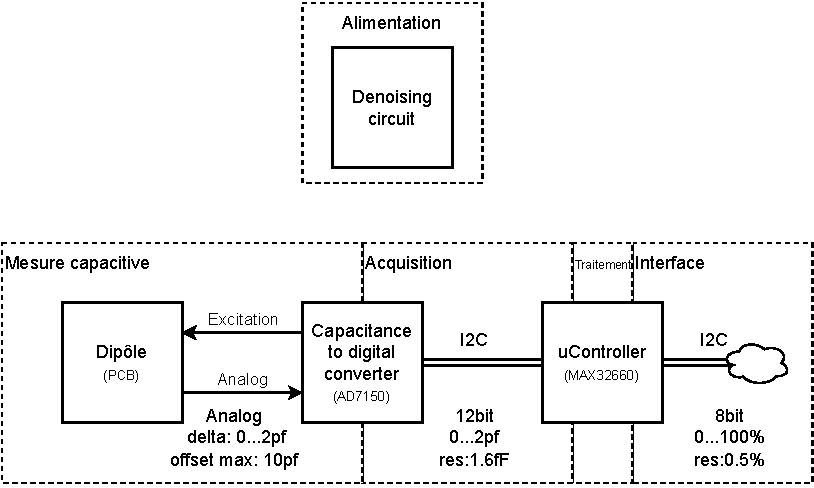
\includegraphics[width=16cm]{SchemaBlock.pdf}
 \caption{Schéma Block}
\end{figure}
